\section{Experiment 4 - Multiobjective EA}
\label{sec:exp4}
In this experiment set the three versions of the Evo-RoleMiner$M$ are tested (see section \ref{sec:EvoRoleMiner}). To counteract on the diversity problem and the strong bias of the complexity measure (role count, assignments counts) in the previous experiments, the Evo-RoleMiner$M$ is tested on the Dataset1 (Experiment 4a-c) and the Healthcare dataset (Experiment 4d-f). For the objectives "Confidentiality Violations" and "Availability Violations" are chosen, since as shown in Experiment 1 the objectives are conflicting (see section \ref{sec:exp1}). The setup can be seen in Table \ref{tab:exp4_setup}.

\begin{table}[H]
	\centering
	\begin{adjustbox}{width=0.75\textwidth}
		\begin{tabular}{|l|l|}
			\hline
			\rowcolor{myGray} 
			\textbf{Parameter}              & \textbf{Value}    \\ \hline
			Generations                     & 100 / 1000 / 2000 \\ \hline
			Population                      & 1000        		\\ \hline
			CXPB                            & 0.25              \\ \hline
			MUTPB-Type1: Add role           & 0.25              \\ \hline
			MUTPB-Type2: Add User           & 0.25              \\ \hline
			MUTPB-Type3: Add Permission     & 0.25              \\ \hline
			MUTPB-Type4: Remove Role        & 0.25              \\ \hline
			MUTPB-Type5: Remove User        & 0.25              \\ \hline
			MUTPB-Type6: Remove Permission  & 0.25              \\ \hline
			Local optimization              & True        		\\ \hline
			Objective 1					    & Confidentiality / Violation Count   \\ \hline
			Objective 2					    & Availability / Assignment Count    	\\ \hline
		\end{tabular}
	\end{adjustbox}
	\caption{EXPERIMENT 4 setup. For experiments 4a-c a generation limit of 100 is chosen, while for experiments 4d-e the generation limit is 2000, experiment f has a limit of 1000. Objective 1 and 2 are confidentiality and availability violations respectively for experiments 4a,b,d,e. For Experiment 4c and f Objective 1 is the sum of confidentiality and availability violations and Objective 2 is the sum of user-role- and role-permission assignments.}
	\label{tab:exp4_setup}
\end{table}

All results can be seen in the Appendix \ref{sec:A_Exp4}. The most interesting results are presented in the following subsections.

\subsection{Evo-RoleMiner$M$ with NSGA-II}
Figure \ref{fig:exp4a_fitness} on the next page shows the development of the population in one of the experiments with Dataset1 (for the Healthcare dataset see Appendix \ref{sec:A_Exp4d_Diagrams}). It can be seen that the individuals in each generation have a wide spread and converging near a pareto front. Since the Dataset1 yields a solution where both objectives can be met, the pareto front consist of one point at (0,0) if the solution is found. The objectives of confidentiality and availability violations are only conflicting until the solution is found.

\begin{figure}[H]
	\centering
	\begin{subfigure}{\textwidth}
		\centering
		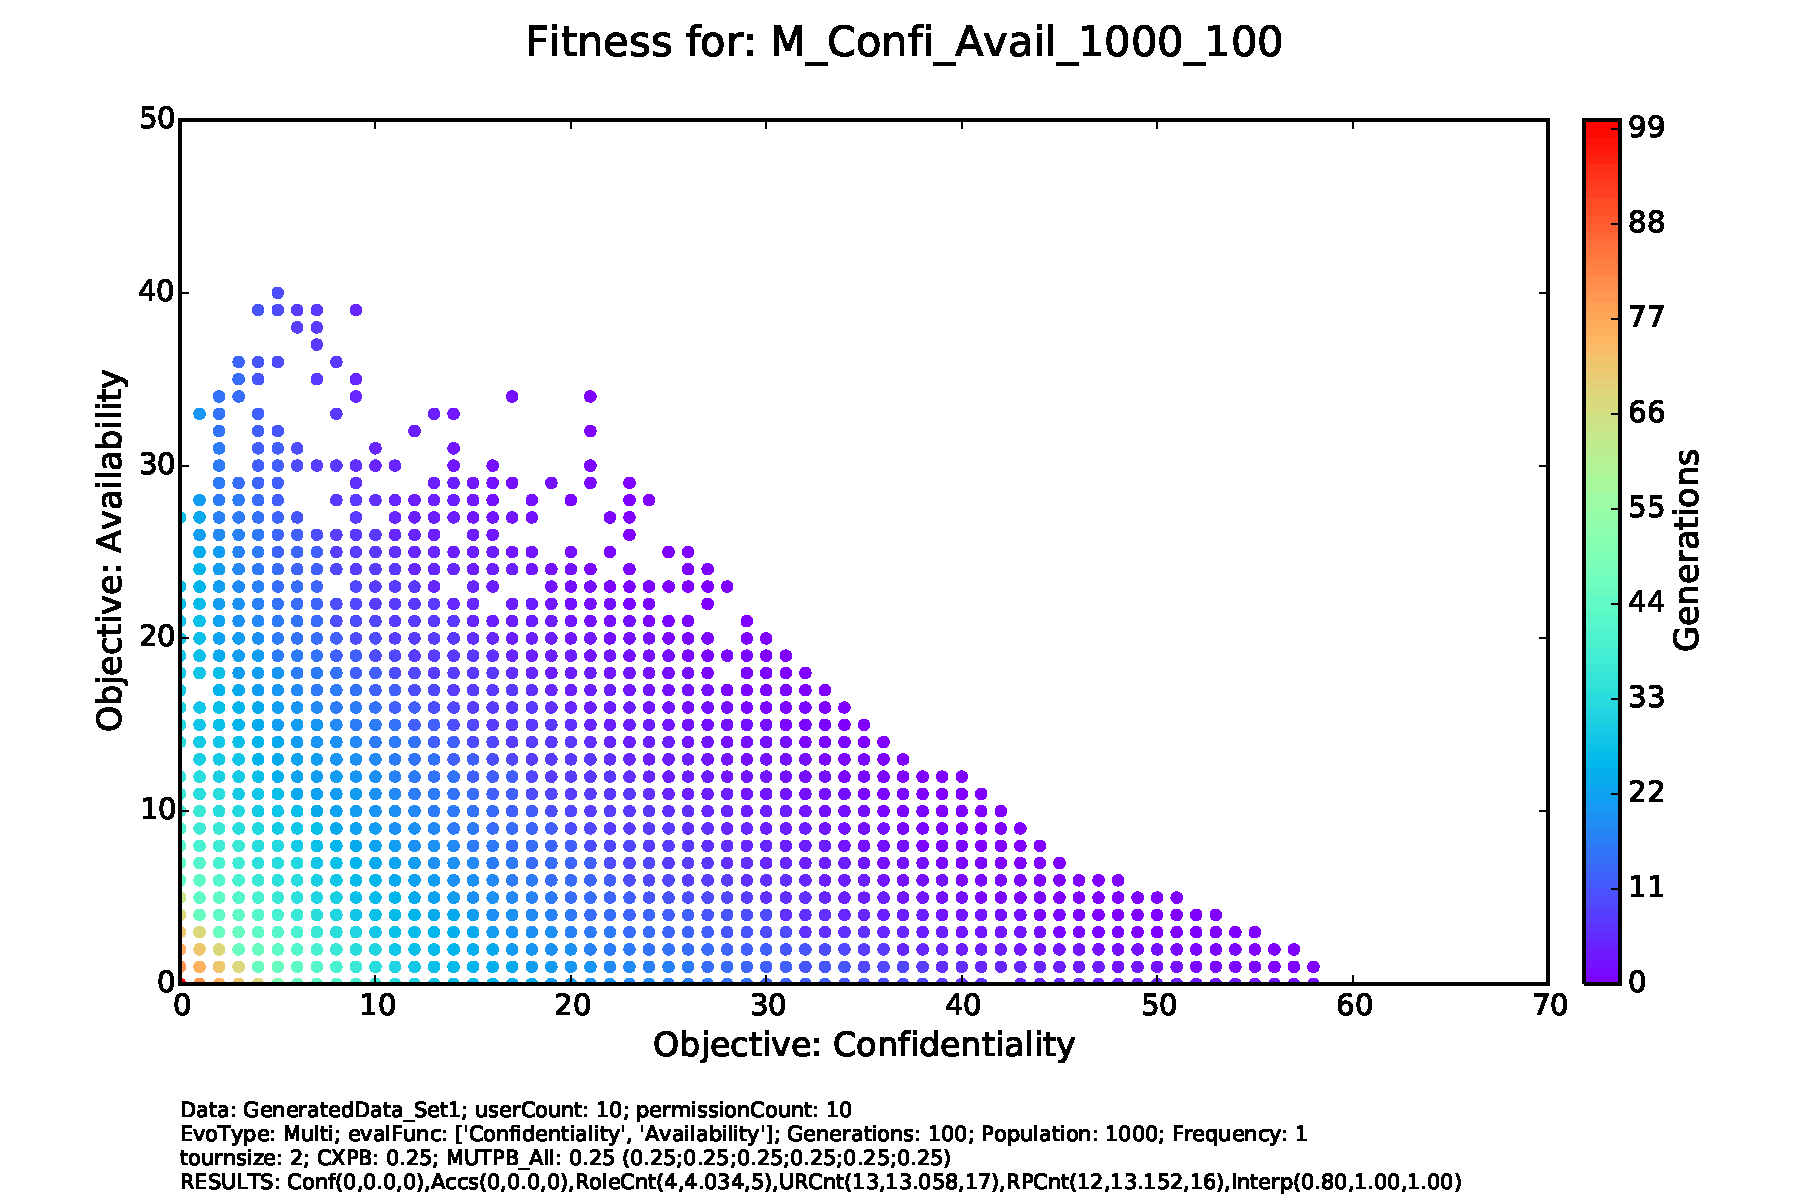
\includegraphics[width=0.8\textwidth, trim=0cm 2cm 0cm 1.5cm, clip=true]{exp4a_fitness}
		\caption{}
		\label{fig:exp4a_fitness_A}
	\end{subfigure}
	\begin{subfigure}{\textwidth}
		\centering
		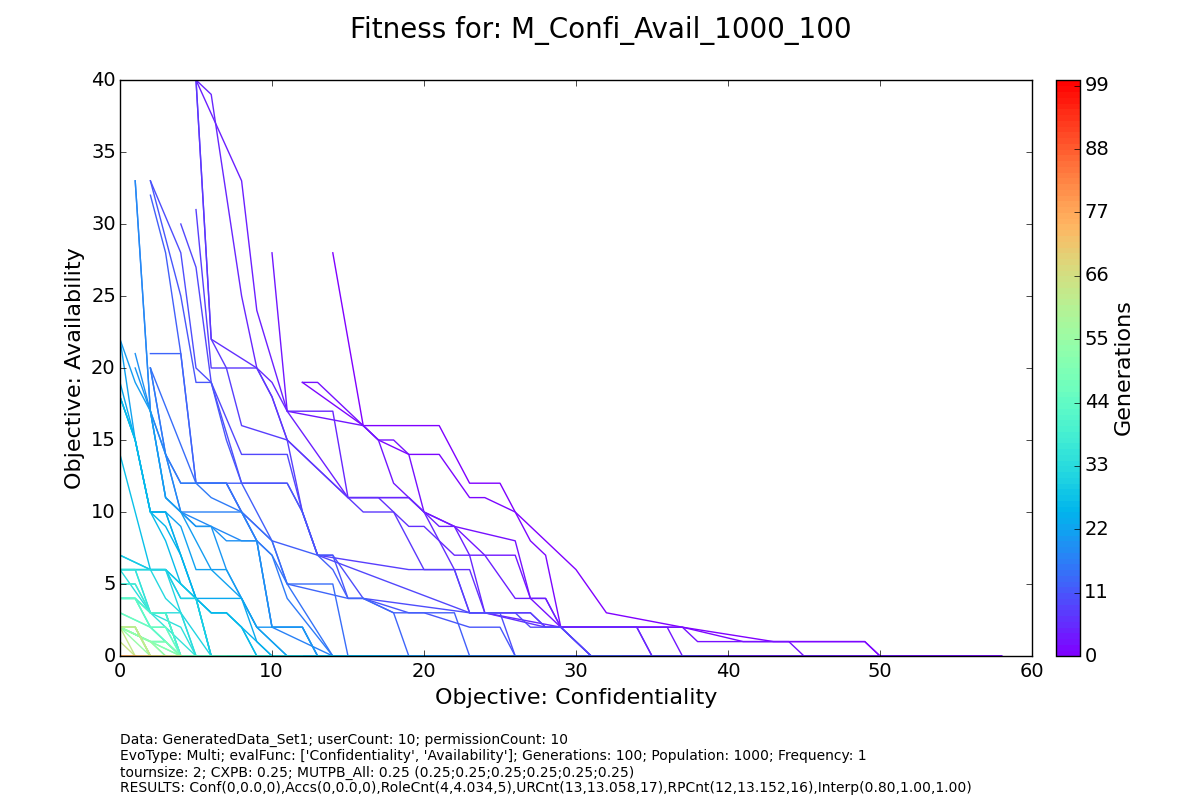
\includegraphics[width=0.8\textwidth, trim=0cm 2cm 0cm 1.5cm, clip=true]{exp4a_fitness_pareto}
		\caption{}
		\label{fig:exp4a_fitness_B}
	\end{subfigure}
	\caption{EXPERIMENT 4a: Example solution of the experiments with Evo-RoleMiner$M$ (based on NSGA-II) on Dataset1. (a) Fitness of individuals over several generations (b) Pareto fronts of each generation.}
	\label{fig:exp4a_fitness}
\end{figure}

An example boxplots on the diversity of the role count of individuals of a population is shown in Figure \ref{fig:exp4d_diversity} for the Healthcare dataset. Compared to the role count diversity in the experiments with the Evo-RoleMiner (see Figure \ref{fig:exp3c_diversity}), the Evo-RoleMiner$M$ allows more diverse role models with different role count. This is owed to the fact that the confidentiality violation objective tends to prefer less roles, while the availability violation objective can be probably better achieved if more roles are existing (see Experiment 1 in section \ref{sec:exp1}).

\begin{figure}[H]
	\centering
	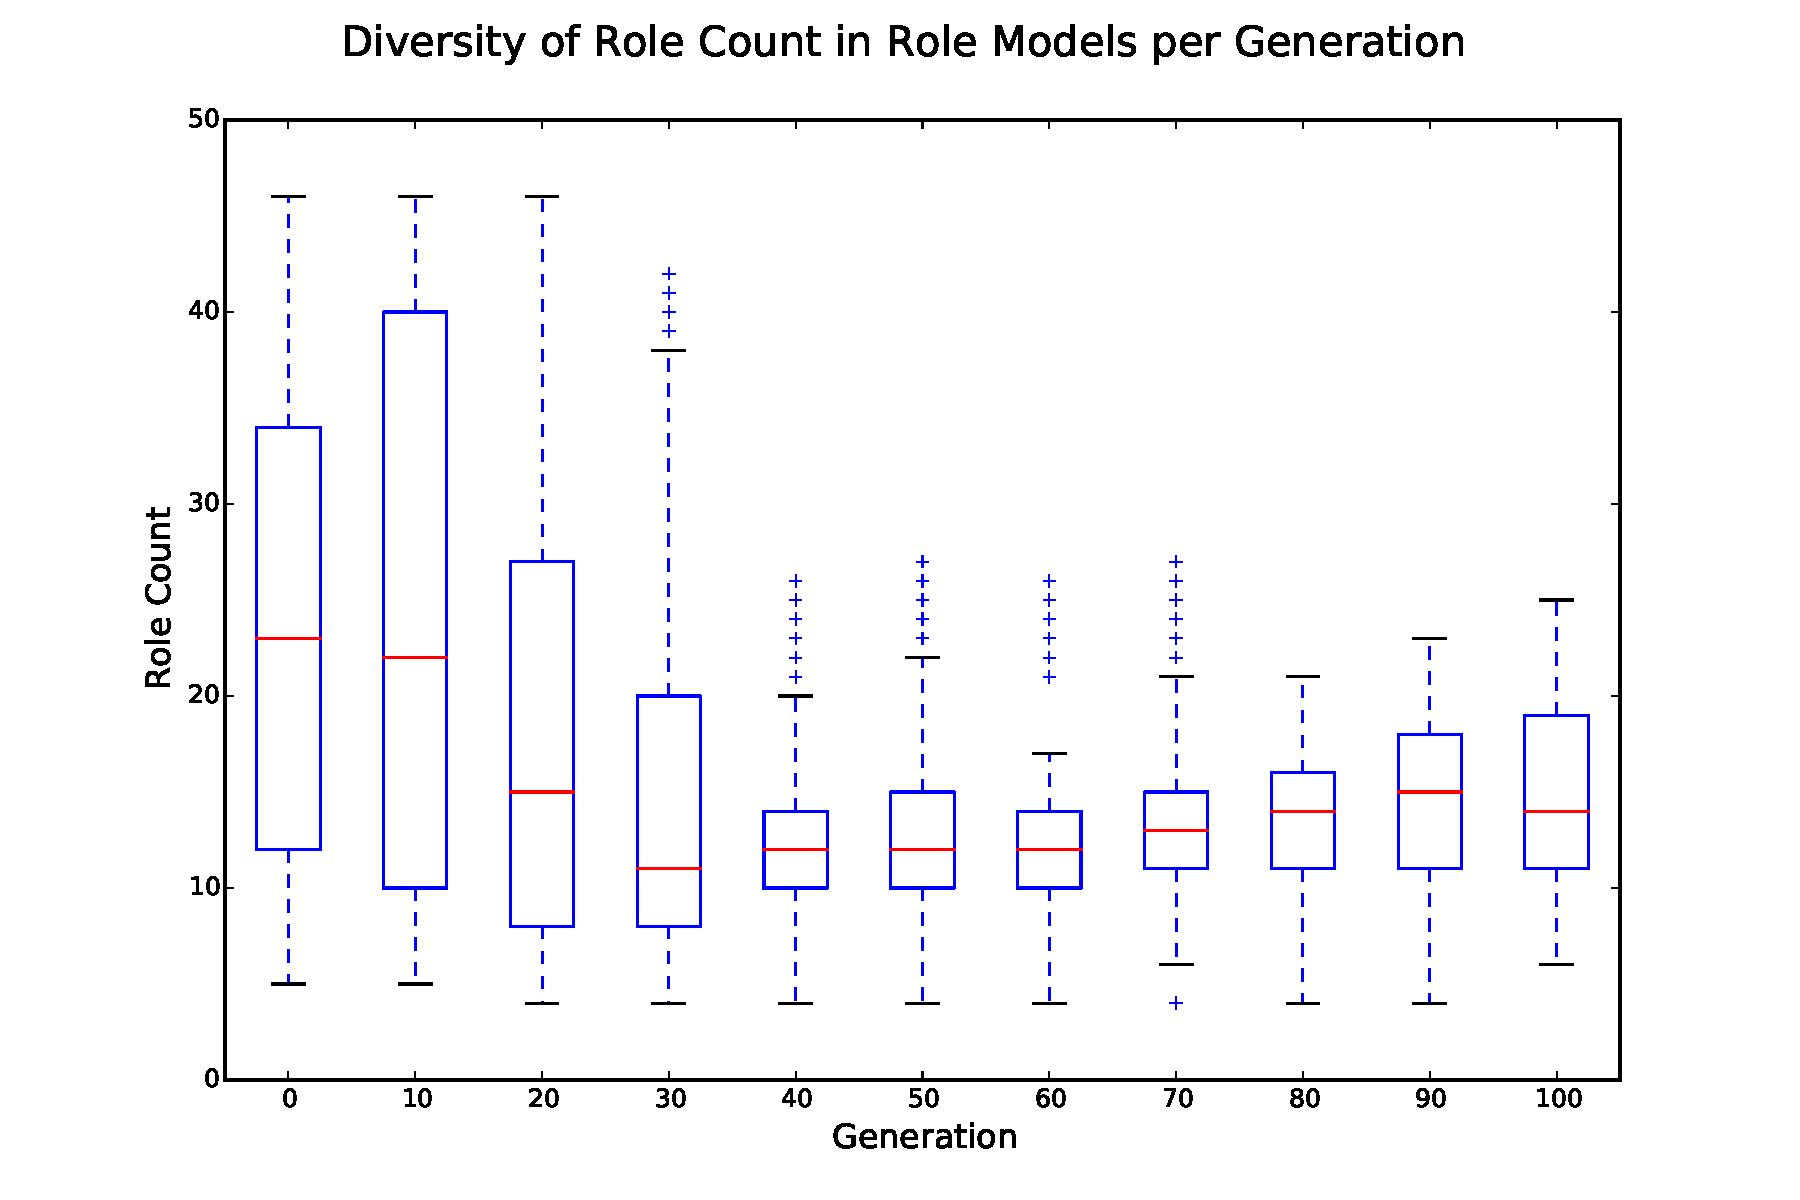
\includegraphics[width=0.7\textwidth]{exp4d_diversity}
	\caption{EXPERIMENT 4d: Example boxplot of role count diversity of individuals of a population in different generations with Evo-RoleMiner$M$ (based on NSGA-II) on the healthcare dataset.}
	\label{fig:exp4d_diversity}
\end{figure}

\subsection{Evo-RoleMiner$M$ with NSGA-II$R$}
Role models can have the same fitness values for both objectives, although their genotype is different (compare for example the role models in Figure \ref{fig:exp4a_RM_compare} on the next page). If several individuals have the same fitness and are in the same non-domination level, they get a crowding distance value of zero (see section \ref{sec:crowdingDistance}). This would imply that role models, who share the same fitness, are favoured in the selection mechanism. Due to this instability in the NSGA-II algorithm, experiment 4b and e are running on a version of the Evo-RoleMiner$M$ based on the improved NSGA-II$R$ algorithm from Fortin et al.\cite{Fortin:2013}. There is a chance that the convergence and diversity of the individuals can be improved, such that the Evo-RoleMiner$M$ can find a solution even faster.

\begin{figure}[H]
	\centering
	\begin{subfigure}[b]{0.5\textwidth}
		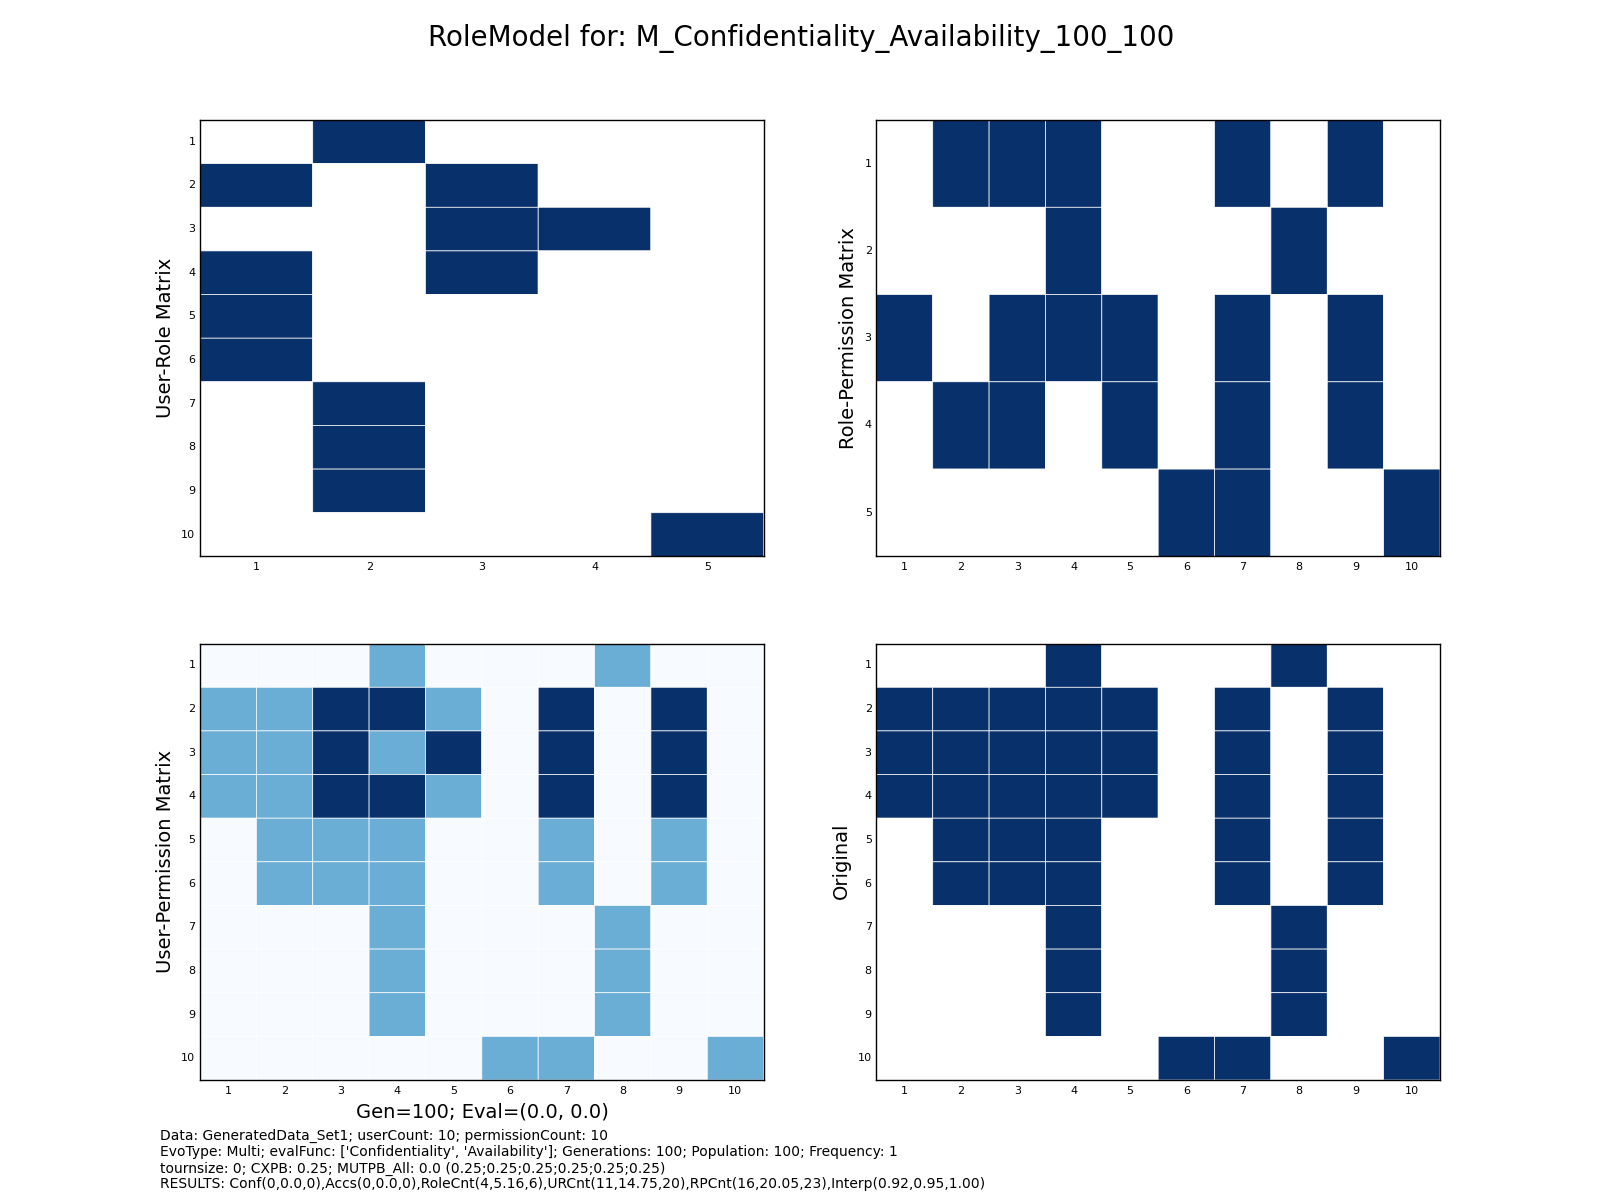
\includegraphics[width=0.9\textwidth,trim=4cm 2cm 4cm 2cm, clip=true]{exp4a_RM}
		\caption{}
		\label{fig:exp4a_RM}
	\end{subfigure}%
	%add desired spacing between images, e. g. ~, \quad, \qquad, \hfill etc. 
	%(or a blank line to force the subfigure onto a new line)
	\begin{subfigure}[b]{0.5\textwidth}
		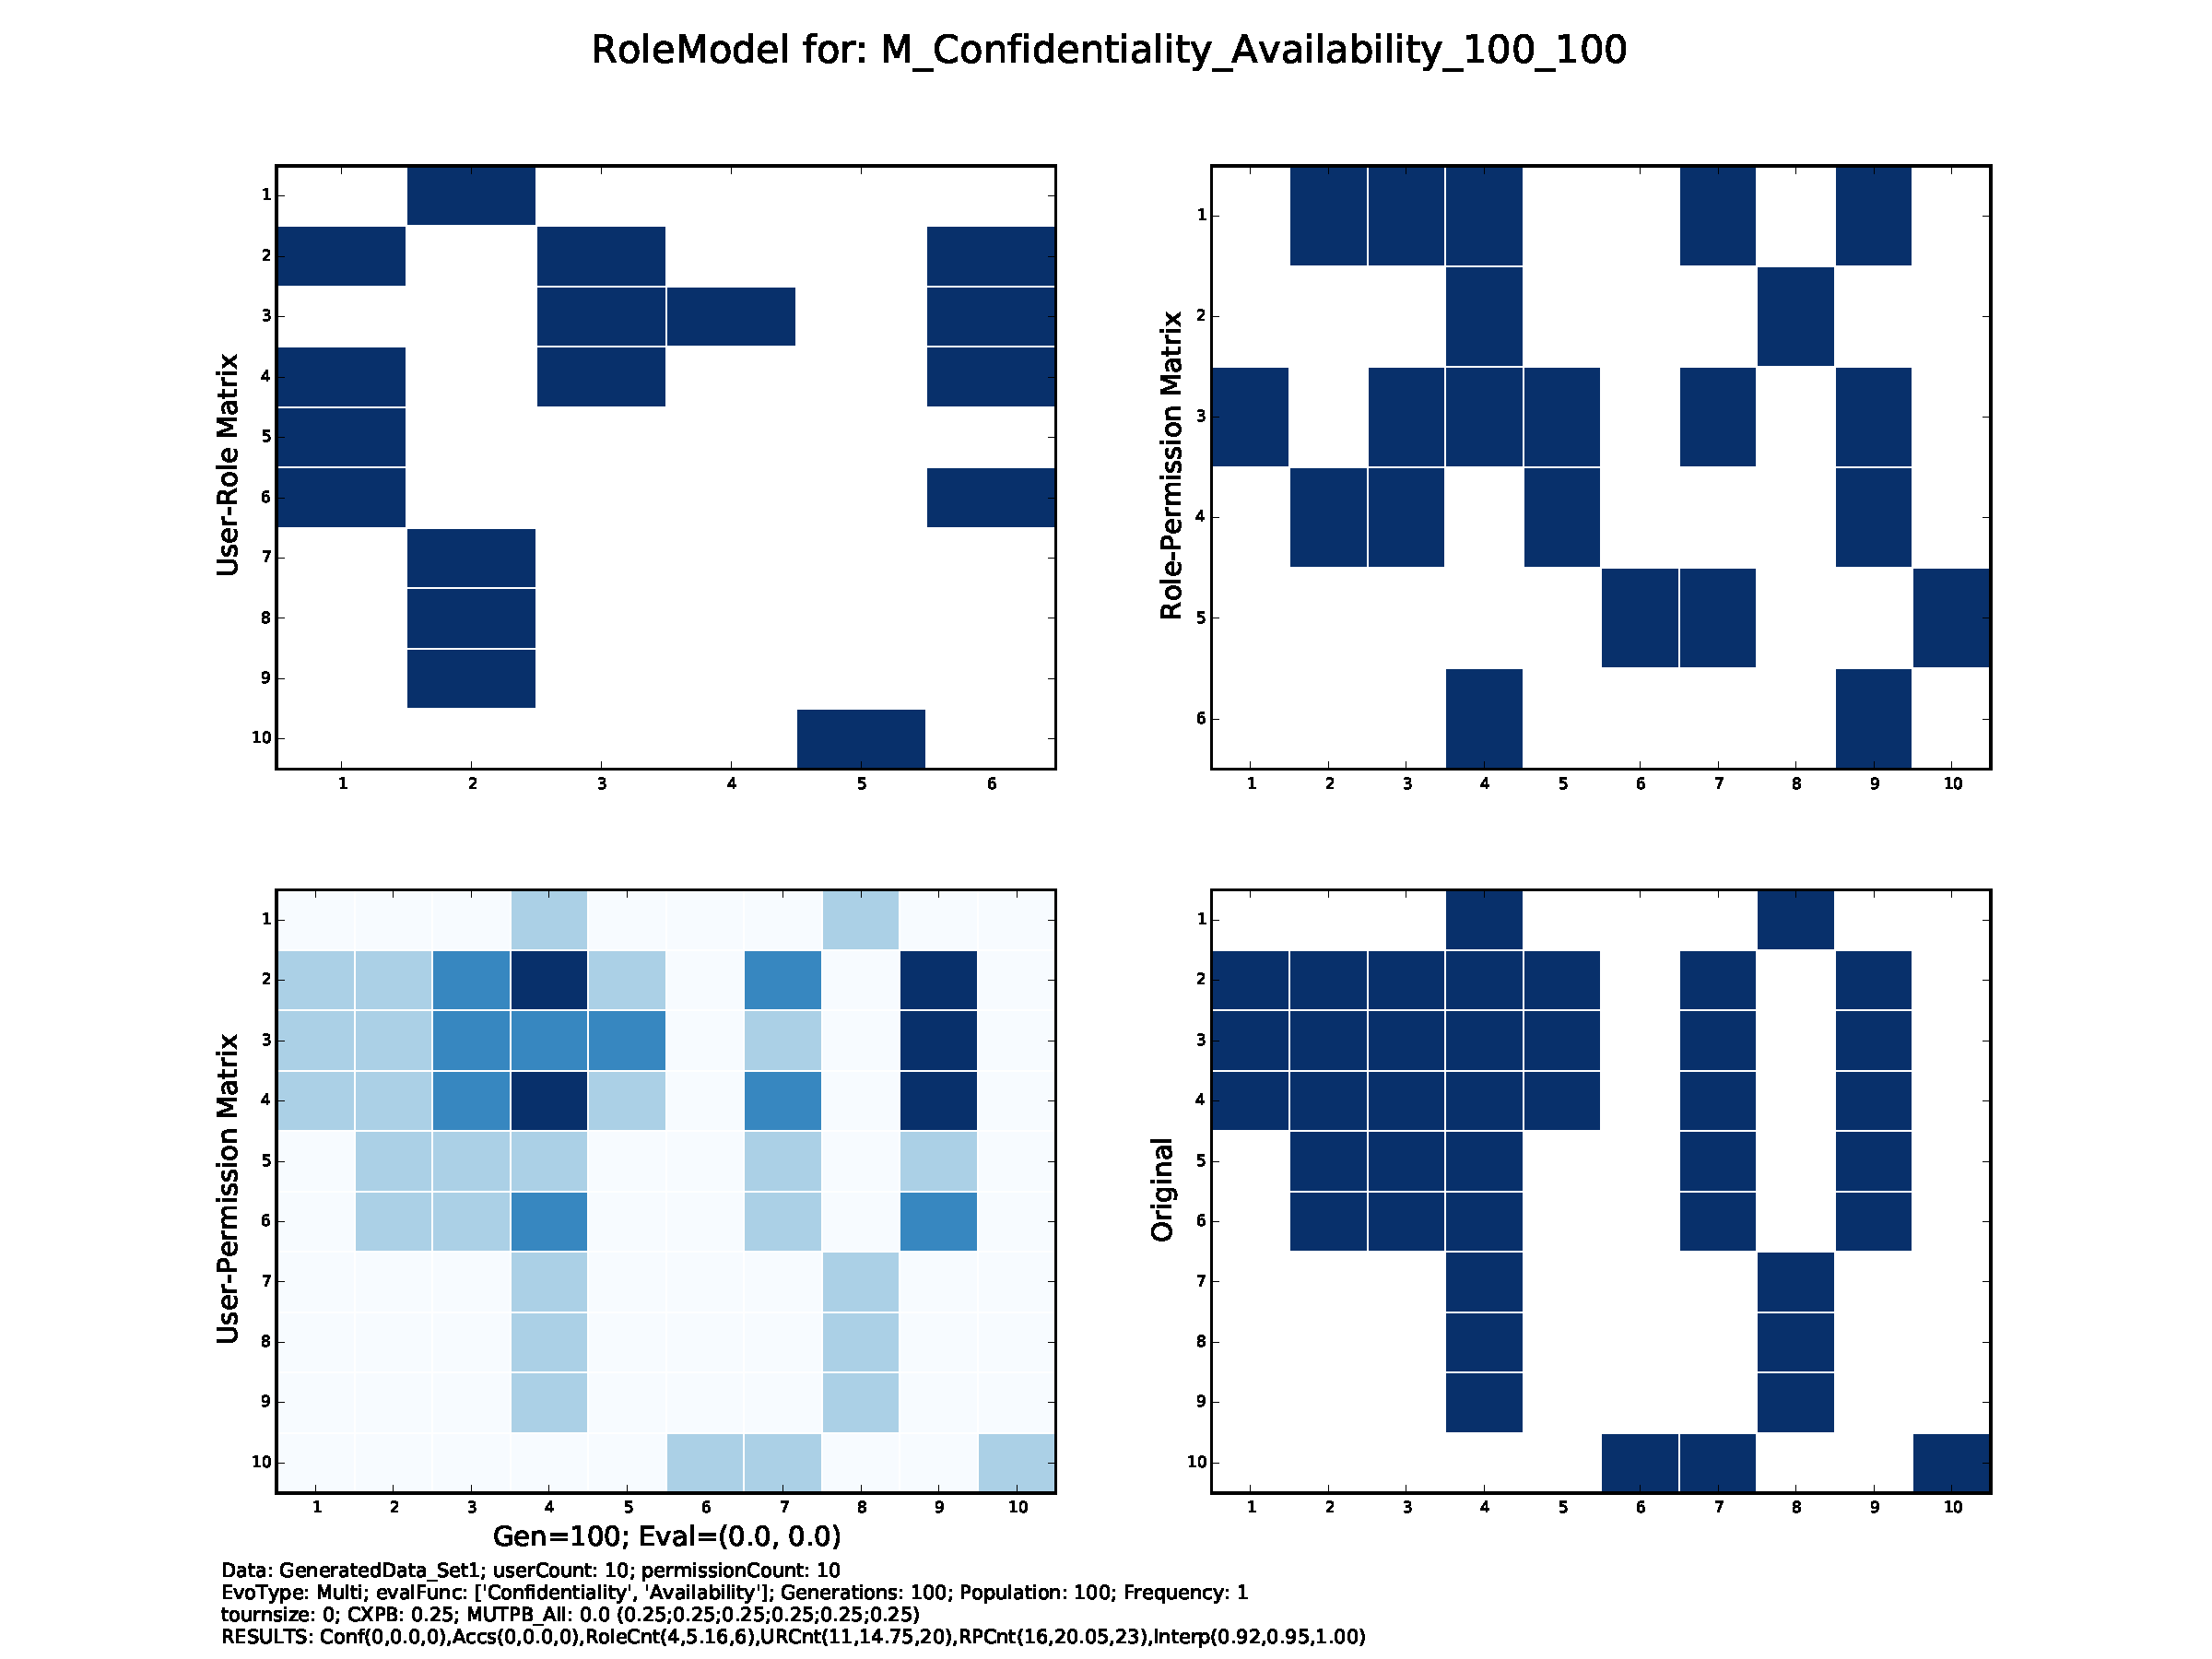
\includegraphics[width=0.9\textwidth, trim=4cm 2cm 4cm 2cm, clip=true]{exp4a_RM2}
		\caption{}
		\label{fig:exp4a_RM2}
	\end{subfigure}
	\caption{EXPERIMENT 4a: Example role models resulting from an experiment on the Evo-RoleMiner$M$ (based on NSGA-II) on Dataset1. For each role model from upper left to lower right: User-Role Matrix, Role-Permission Matrix, Resulting User-Permission Matrix, Original User-Permission Matrix from Input. A blue box stands for an assignment. The darker the blue the more user-role- and role-permission assignments causing the user-permission assignment.}
	\label{fig:exp4a_RM_compare}
\end{figure}

\begin{figure}[H]
	\centering
	\begin{subfigure}{0.5\textwidth}
		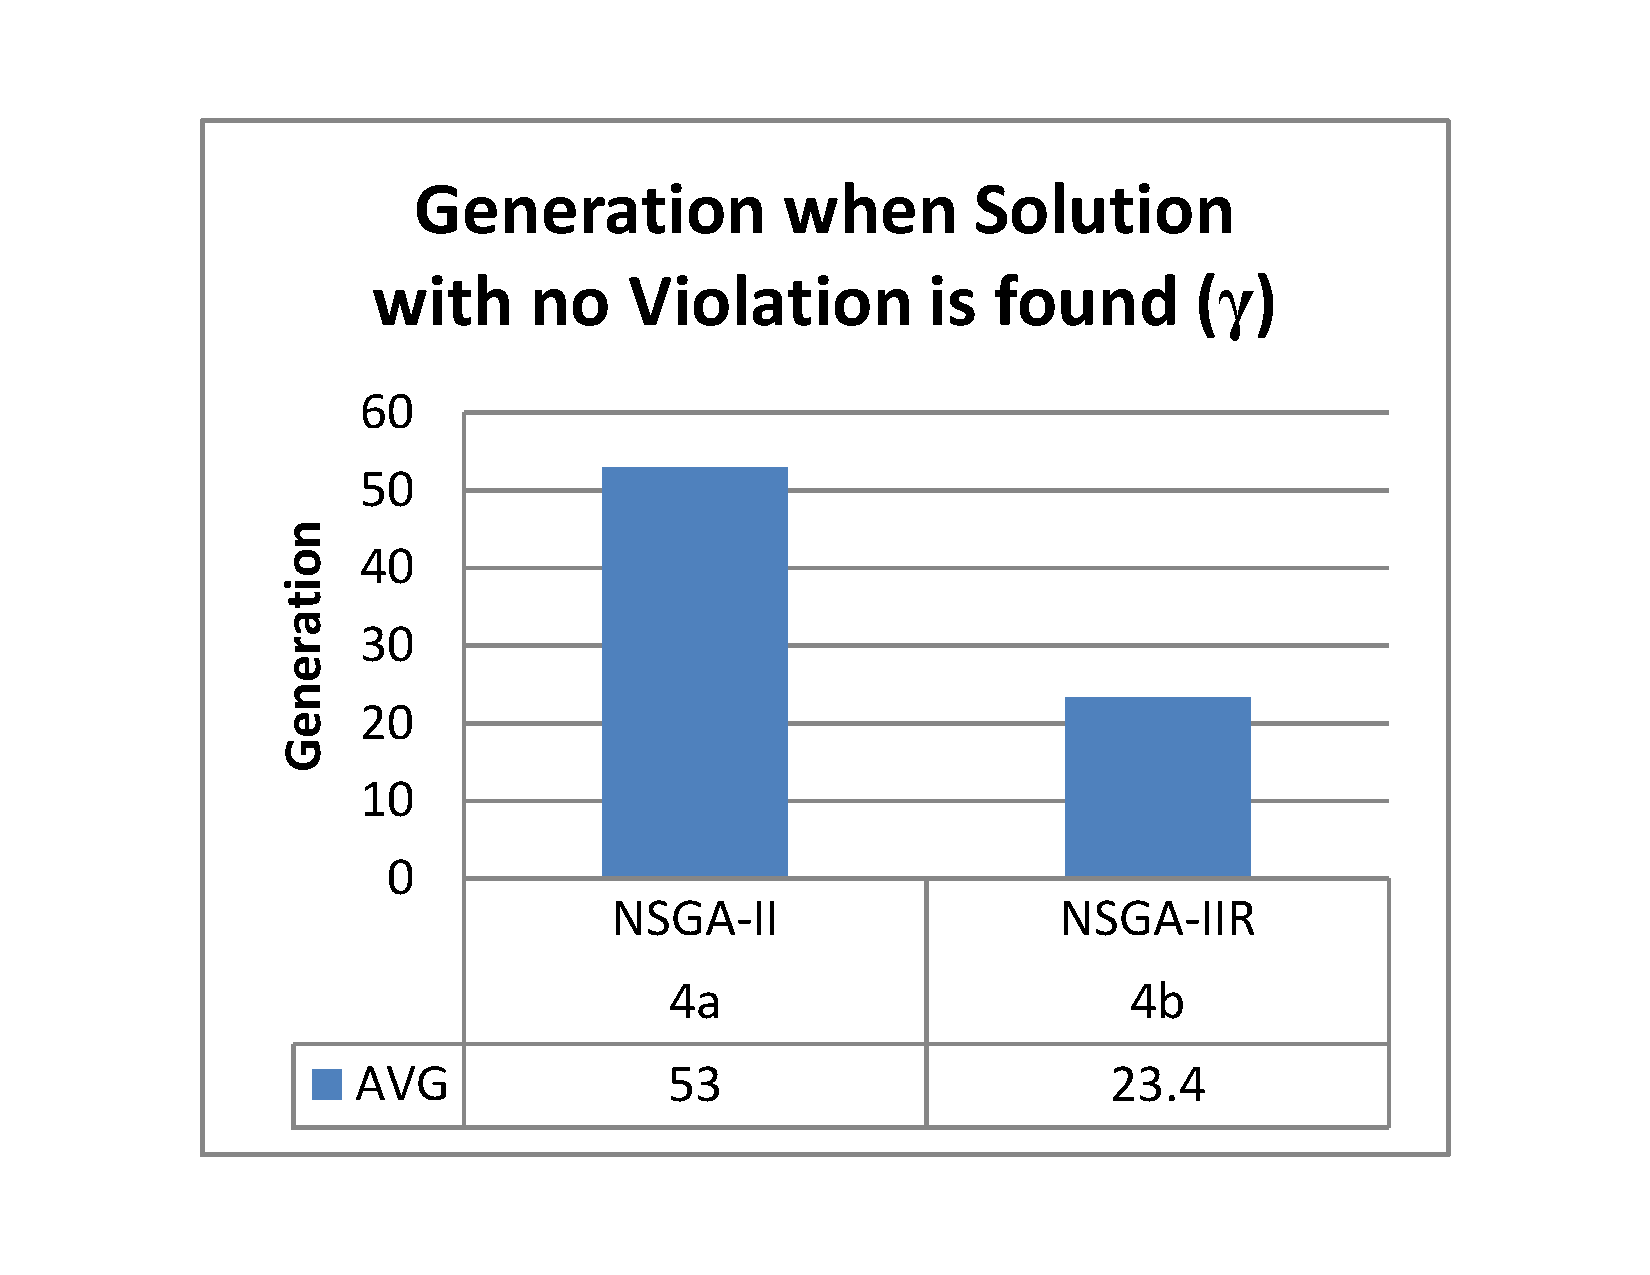
\includegraphics[width=\textwidth]{Results_Exp4b_Gamma_Dataset1}
		\caption{}
		\label{fig:Results_Exp4b_Gamma_Dataset1}
	\end{subfigure}%
	\begin{subfigure}{0.5\textwidth}
		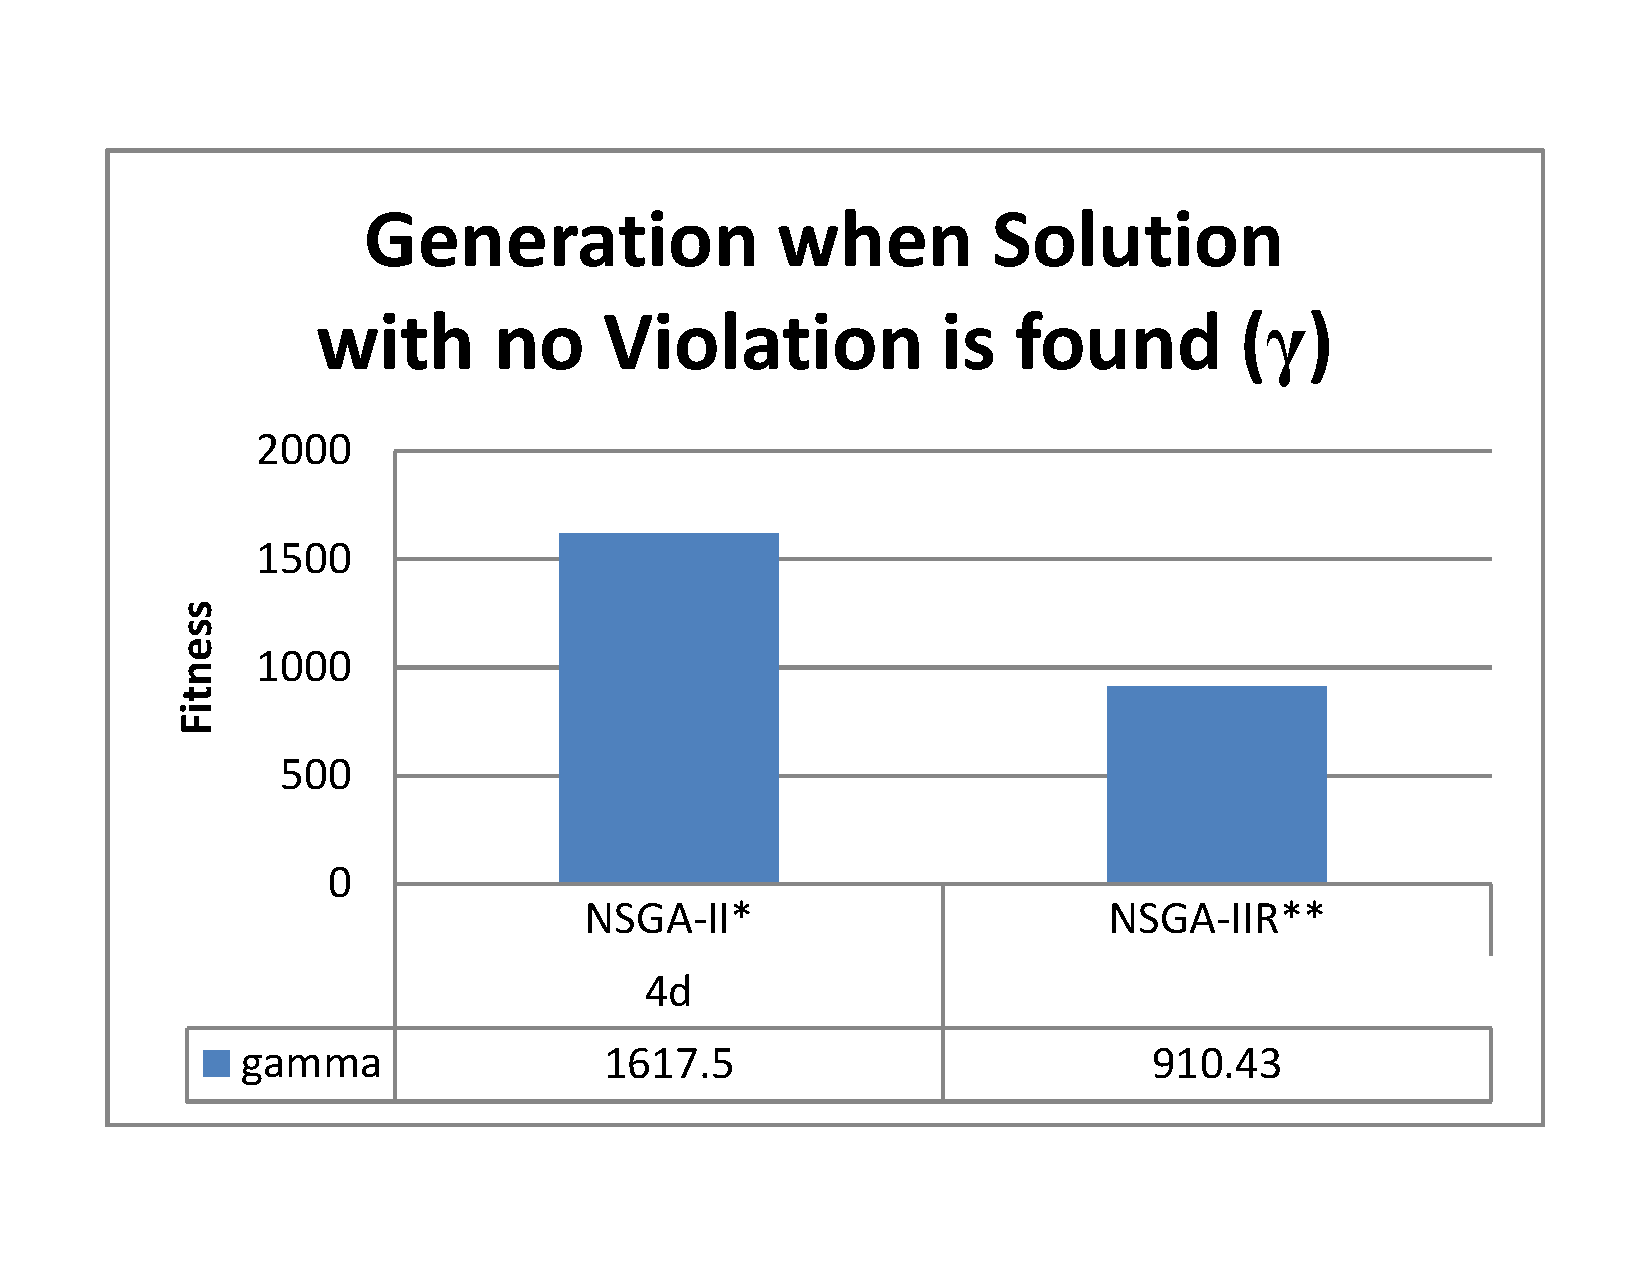
\includegraphics[width=\textwidth]{Results_Exp4f_Healthcare_Gamma}
		\caption{*NSGA-II: Solution found in 4 experiments; **NSGA-II$R$: Solution found in 7 experiments)}
		\label{fig:Results_Exp4f_Healthcare_Gamma}
	\end{subfigure}
	\caption{Comparison of Evo-RoleMiner$M$ based on NSGA-II and on based on NSGA-II$R$. It shows the average generation when a solution with no confidentiality or availability violations is found. (a) for Dataset1 (b) for Healthcare Dataset}
	\label{fig:Results_Exp4b_f_Gamma}
\end{figure}

In case of Dataset1 (Experiment 4b) it can be seen that the Evo-RoleMiner$M$ based on NSGA-II$R$ gives an improvement, since in average a solution with no violations is found after 23.4 generations, while in case of the Evo-RoleMiner$M$ based on the traditional NSGA-II, the average generation when a solution is found is 53 (see Figure \ref{fig:Results_Exp4b_Gamma_Dataset1}). Also a T-Test confirmed a statistical significant difference (P-Value in T-Test is less than 0.0001).

In case of the Healthcare dataset (Experiment 4e) after 1000 Generations no solution with no violations is found with Evo-RoleMiner$M$ based on NSGA-II. Applying Evo-RoleMiner$M$ based on NSGA-II$R$ a solution with no violations could be found in five of the 10 experiments, where the average generation is 757.8.

\begin{figure}[H]
	\centering
	\begin{subfigure}{\textwidth}
		\centering
		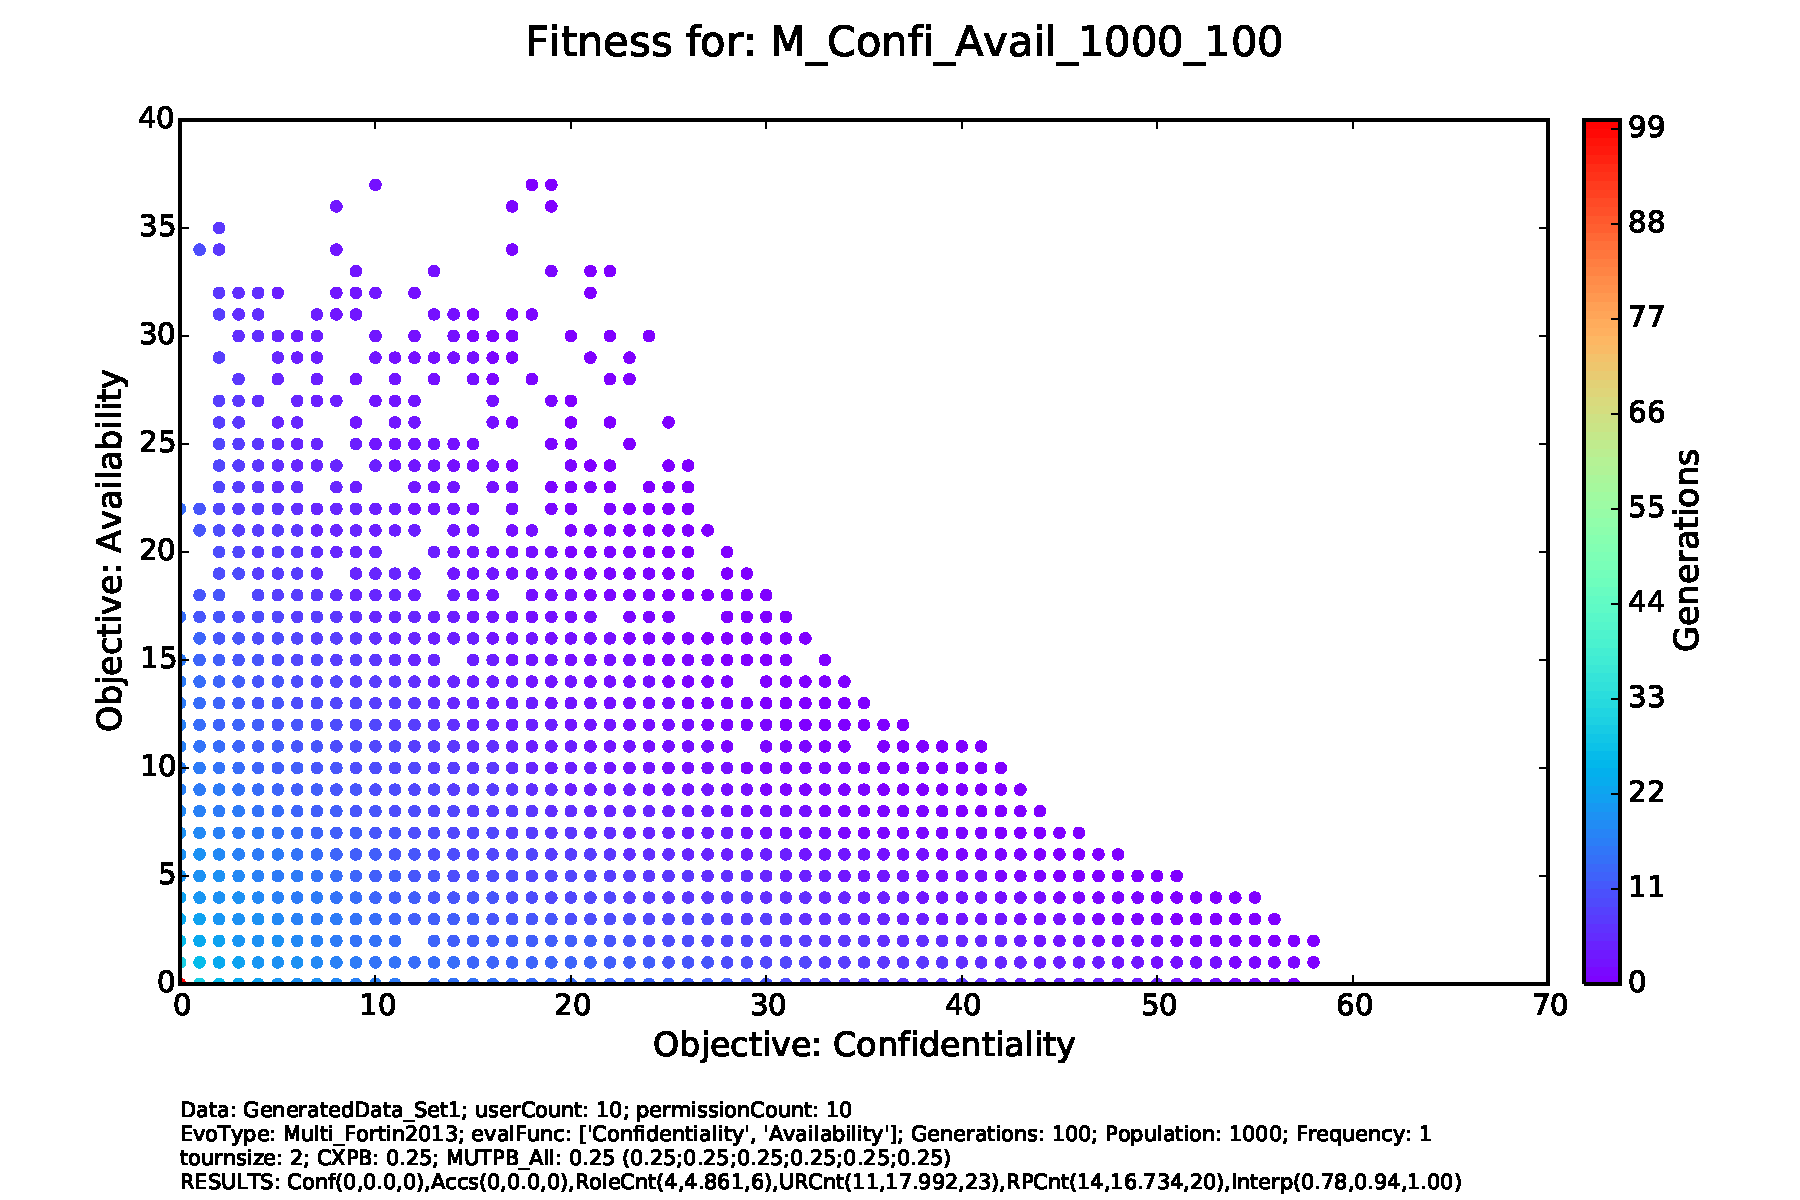
\includegraphics[width=0.8\textwidth, trim=0cm 2cm 0cm 1.5cm, clip=true]{exp4b_fitness}
		\caption{}
		\label{fig:exp4b_fitness_A}
	\end{subfigure}
	\begin{subfigure}{\textwidth}
		\centering
		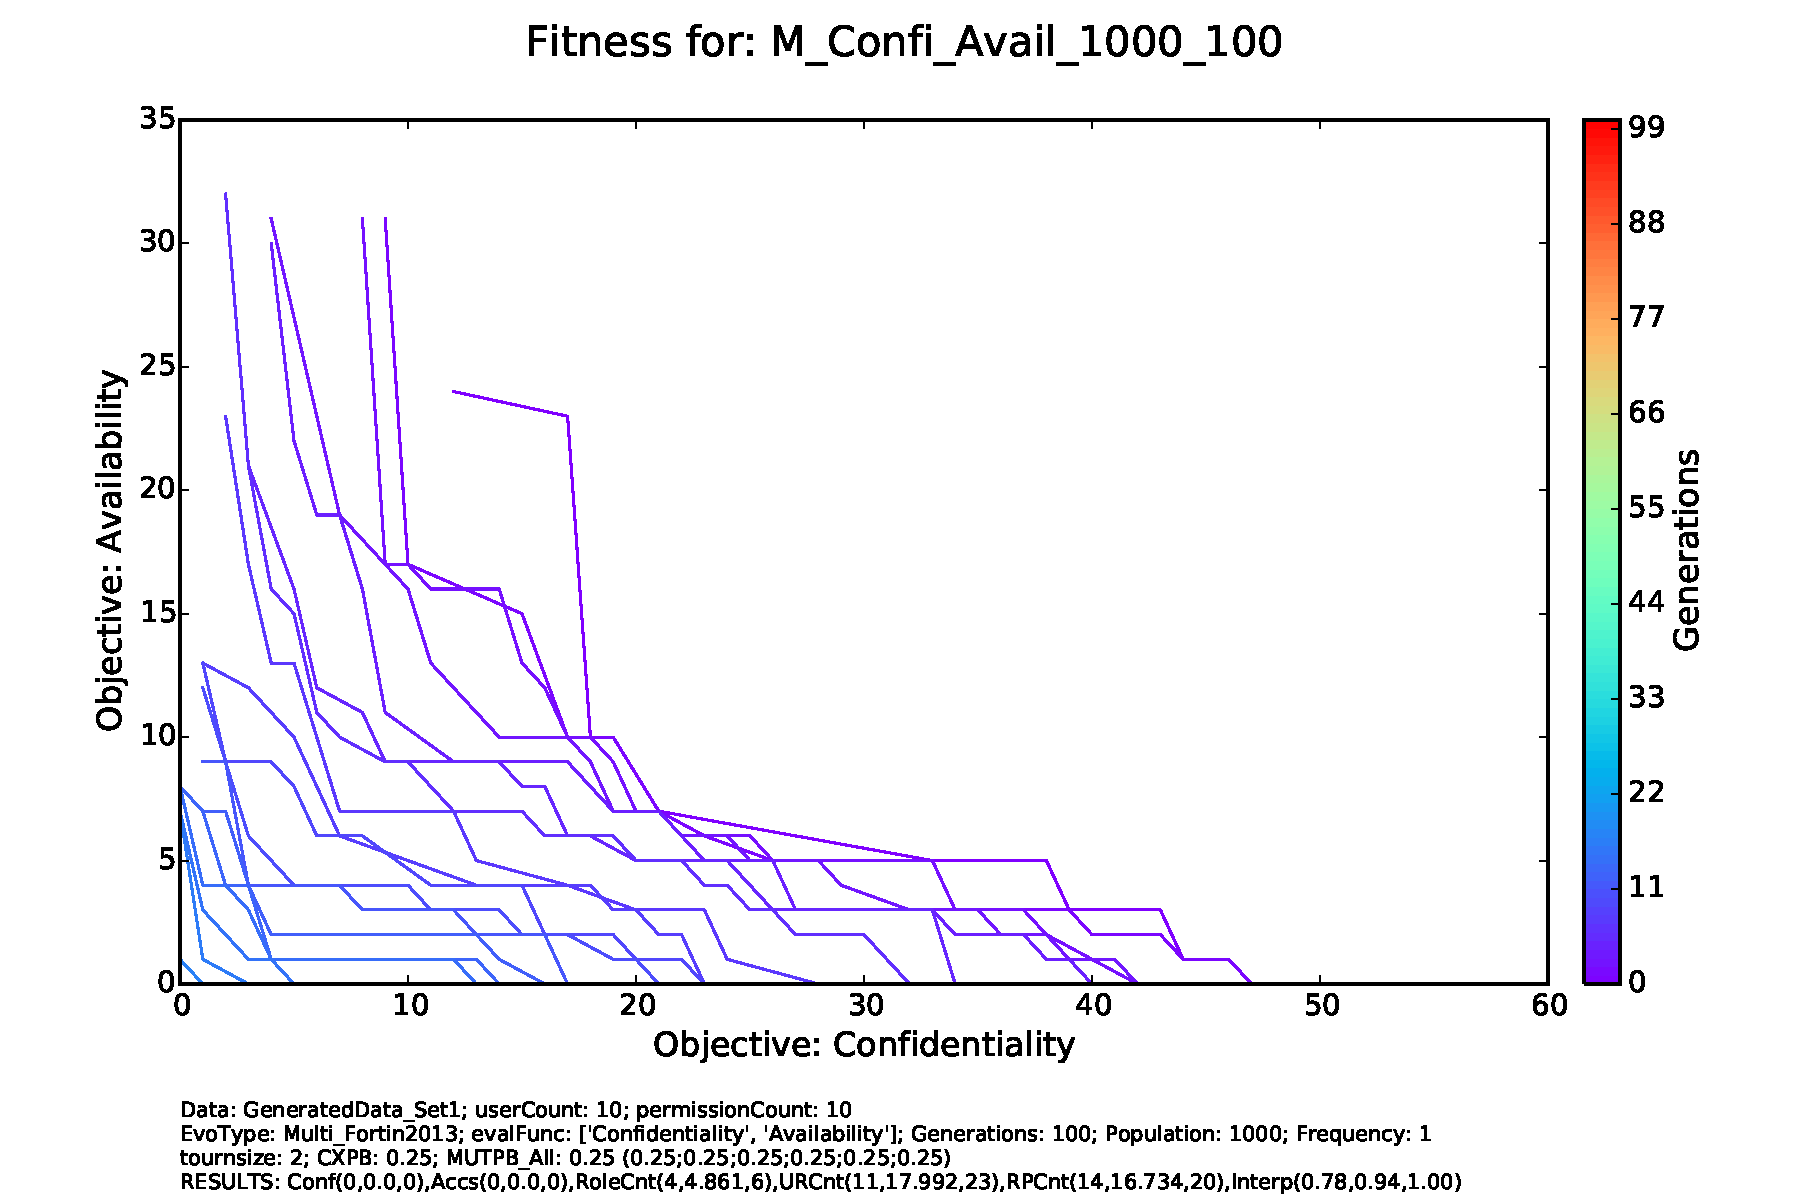
\includegraphics[width=0.8\textwidth, trim=0cm 2cm 0cm 1.5cm, clip=true]{exp4b_fitness_pareto}
		\caption{}
		\label{fig:exp4b_fitness_B}
	\end{subfigure}
	\caption{EXPERIMENT 4b: Example solution of the experiments with Evo-RoleMiner$M$ based on NSGA-II$R$ on Dataset1. (a) Fitness of individuals over several generations (b) Pareto fronts of each generation.}
	\label{fig:exp4b_fitness}
\end{figure}


\subsection{Evo-RoleMiner$M$ with NSGA-II$R$ with weights}
\label{sec:exp_nsga2rweights}
The objectives chosen for experiment 4a,b,d,e are only confidentiality and availability violations. Although the local optimization (see section \ref{sec:localOptimization}) is preventing roles with the same user- or permission-assignments, the Evo-RoleMiner$M$ cannot distinguish between the complexity of role models, which can reconstruct the original access control policy $UPA$. The Basic-RMP optimizes the complexity regards the role count, while the Min-Edge-RMP optimizes towards a minimum user- and permission assignment count.

In experiment 4c and f a third version of the Evo-RoleMiner$M$ is tested, where one objective is the minimization of the combined violations count $|G_{conf} + G_{accs}|$ and the second objective is the minimization of user- and permission assignment count $|UA + PA|$. Since it is known from previous experiments, that the complexity measure has a strong influence the third version of the Evo-RoleMiner$M$ is chosen, which allows to lower the selection pressure on the second objective by setting a probability (see section \ref{sec:weightedNSGA2}). The probability for the second objective is set to 0.8.

The results can be seen in Figure \ref{fig:Results_Exp4} in comparison with the Evo-RoleMiner$M$ based on NSGA-II$R$ without weights and objectives "Confidentiality" and "Availability". In Figure \ref{fig:exp4c_fitness} the development of one of the ten experiments with Evo-RoleMiner$M$ based on NSGA-II$R$ with weights is illustrated.

\begin{figure}[H]
	\centering
	\begin{subfigure}{0.45\textwidth}
		%\centering
		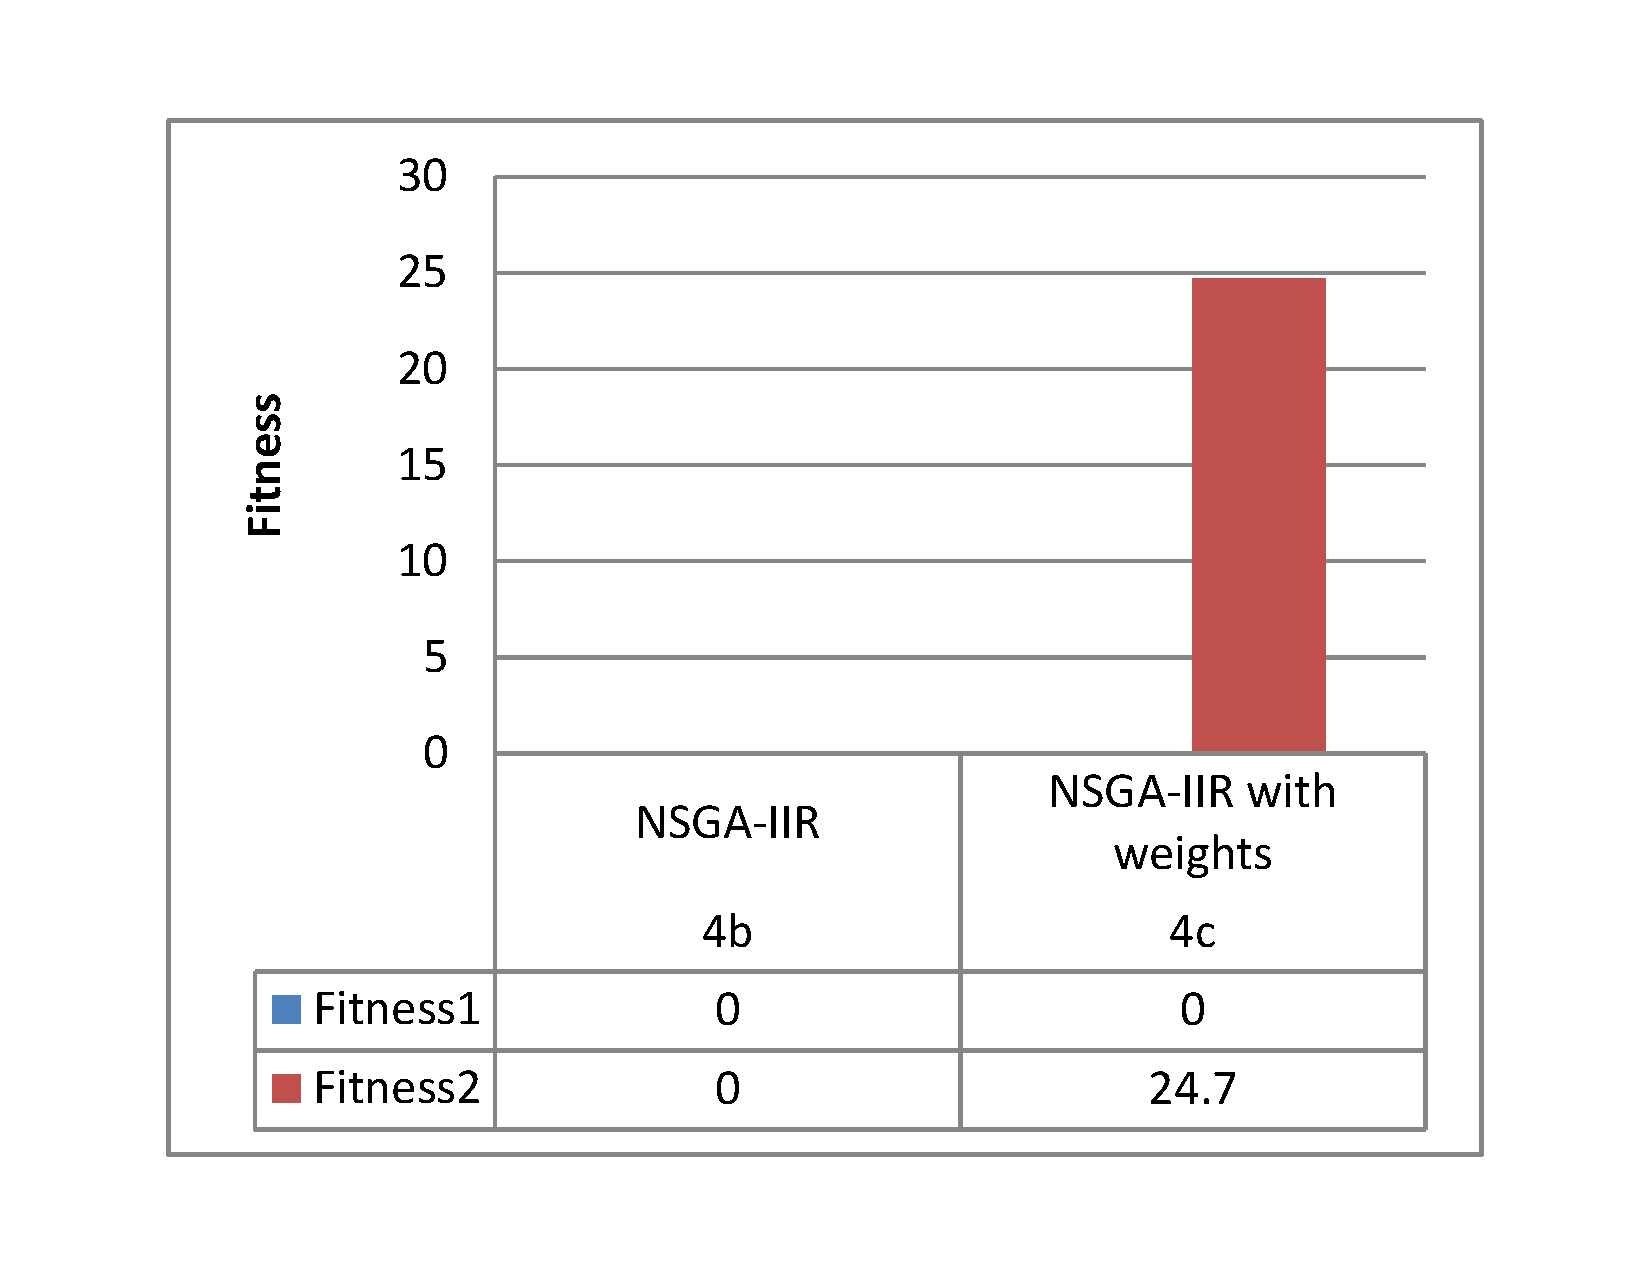
\includegraphics[width=\textwidth, trim=2cm 2cm 2cm 1.5cm, clip=true]{Results_Exp4c_Dataset1_Fitness}
		\caption{Dataset1}
		\label{fig:Results_Exp4c_Dataset1_Fitness}
	\end{subfigure}%
	\begin{subfigure}{0.55\textwidth}
		\centering
		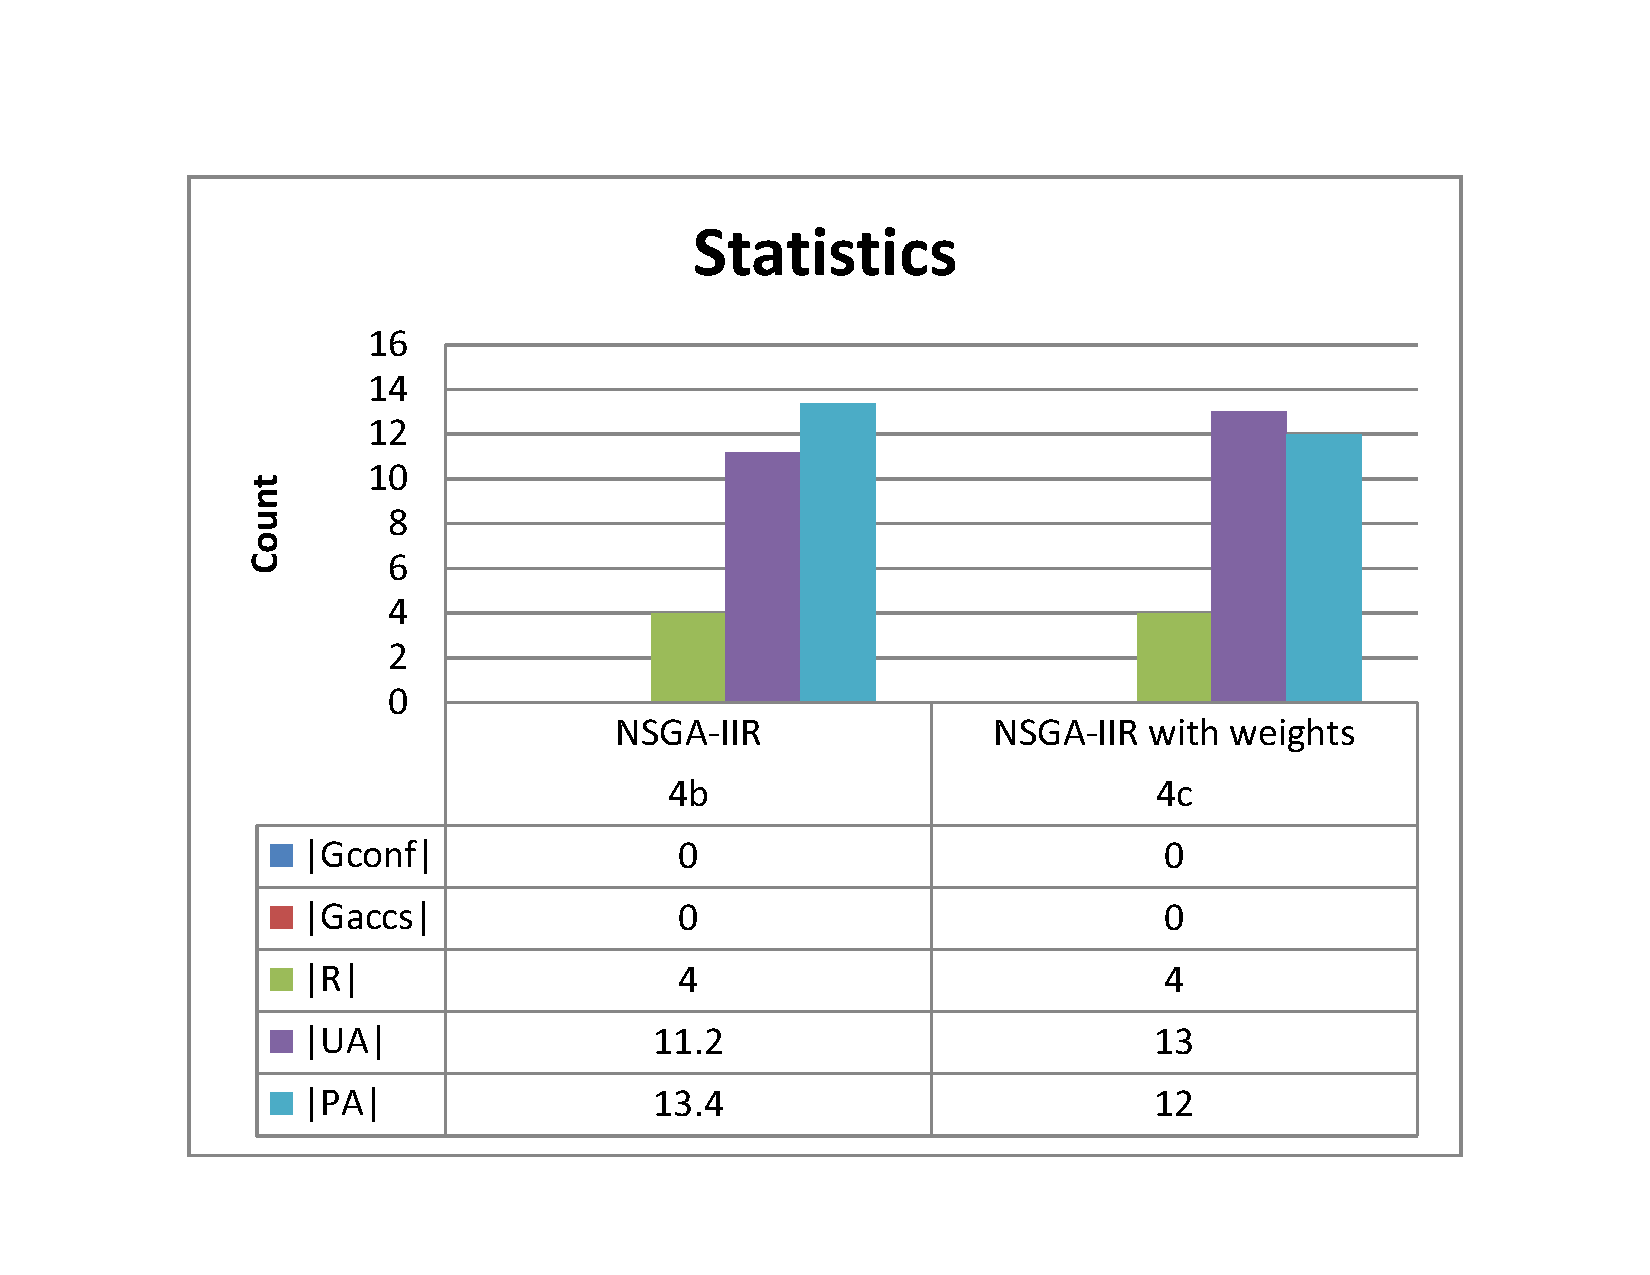
\includegraphics[width=\textwidth, trim=2cm 2cm 2cm 1.5cm, clip=true]{Results_Exp4c_Dataset1_Statistics}
		\caption{Dataset1}
		\label{fig:Results_Exp4c_Dataset1_Statistics}
	\end{subfigure}
	\begin{subfigure}{0.45\textwidth}
		%\centering
		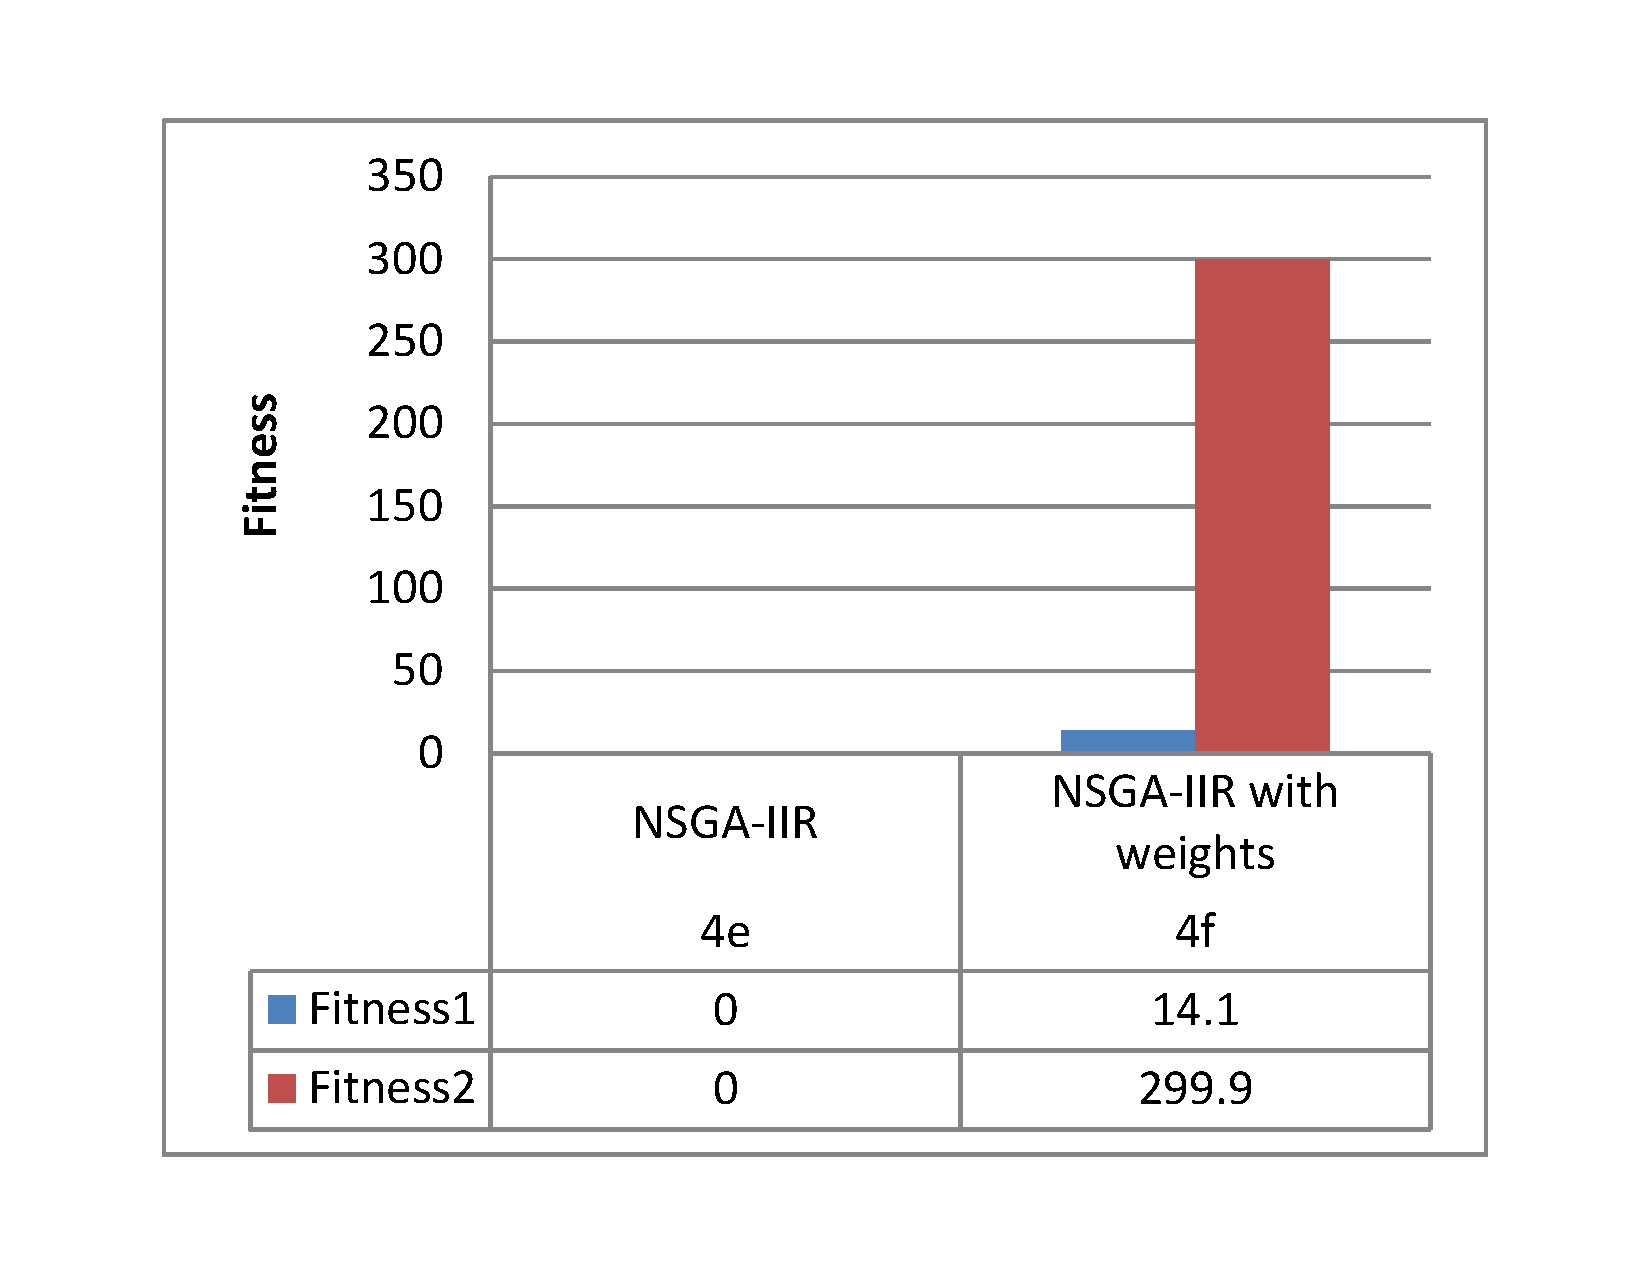
\includegraphics[width=\textwidth, trim=2cm 2cm 2cm 1.5cm, clip=true]{Results_Exp4f_Healthcare_Fitness}
		\caption{Healthcare}
		\label{fig:Results_Exp4f_Healthcare_Fitness}
	\end{subfigure}%
	\begin{subfigure}{0.55\textwidth}
		\centering
		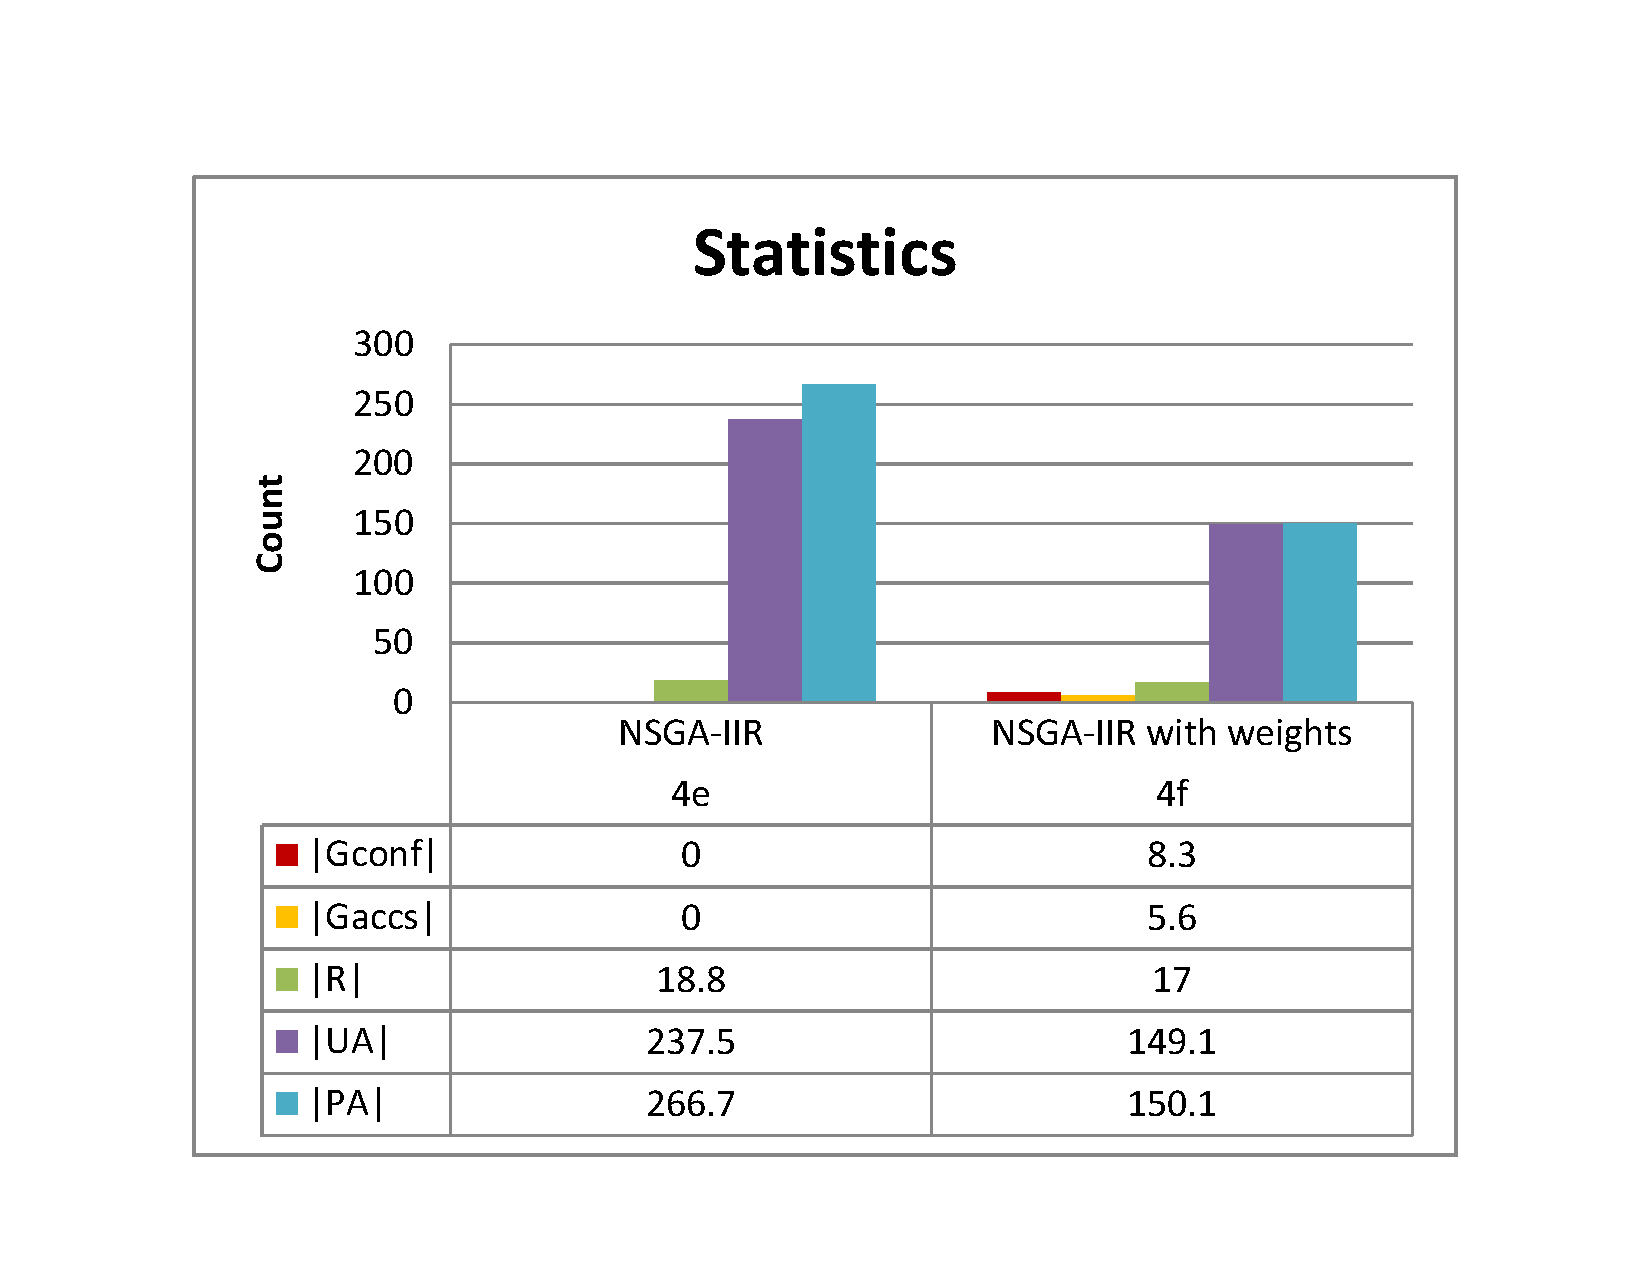
\includegraphics[width=\textwidth, trim=2cm 2cm 2cm 1cm, clip=true]{Results_Exp4f_Healthcare_Statistics}
		\caption{Healthcare}
		\label{fig:Results_Exp4f_Healthcare_Statistics}
	\end{subfigure}
	\caption{EXPERIMENT4b,c,e,f: Statistics of ten experiments with the Evo-RoleMiner$M$ with setup in Table \ref{tab:exp3_setup} for Dataset1 and Healthcare dataset. The values for Fitness, Confidentiality violations ($|G_{conf}|$), Availability violations ($|G_{accs}|$), Roles ($|R|$), User-Role-Assignments ($|UA|$) and Role-Permission assignments ($|PA|$) are the average minimum in the last generation of all experiments.}
	\label{fig:Results_Exp4}
\end{figure}

The results show that the third version of Evo-RoleMiner$M$ less likely finds a violation-free role model than the second version of Evo-RoleMiner$M$. On the other hand on the experiments on the Healthcare dataset, it can be seen that the count of user-role- and role-permission assignments is significantly lower when using the third version of Evo-RoleMiner$M$ (see Figure \ref{fig:Results_Exp4}).\todo[]{T-Test missing}

\begin{figure}[H]
	\centering
	\begin{subfigure}{\textwidth}
		\centering
		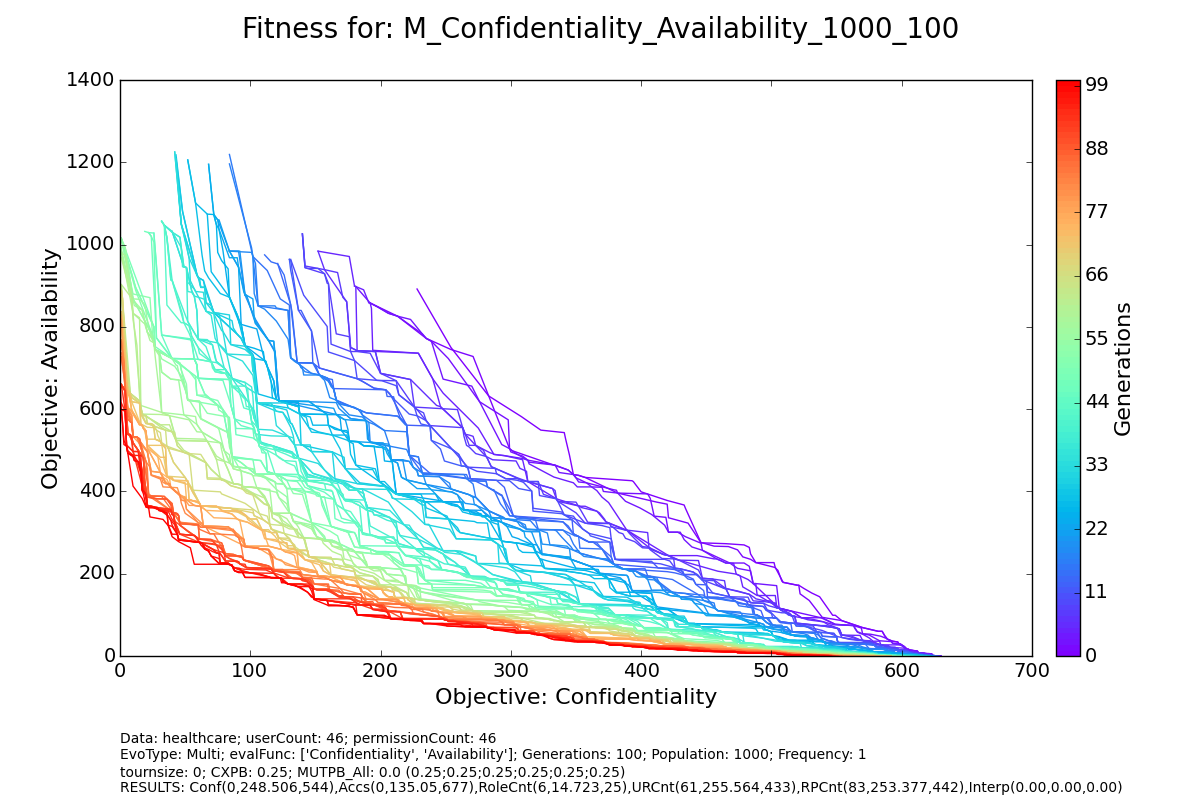
\includegraphics[width=0.8\textwidth, trim=0cm 2cm 0cm 1.5cm, clip=true]{exp4c_fitness}
		\caption{}
		\label{fig:exp4c_fitness_A}
	\end{subfigure}
	\begin{subfigure}{\textwidth}
		\centering
		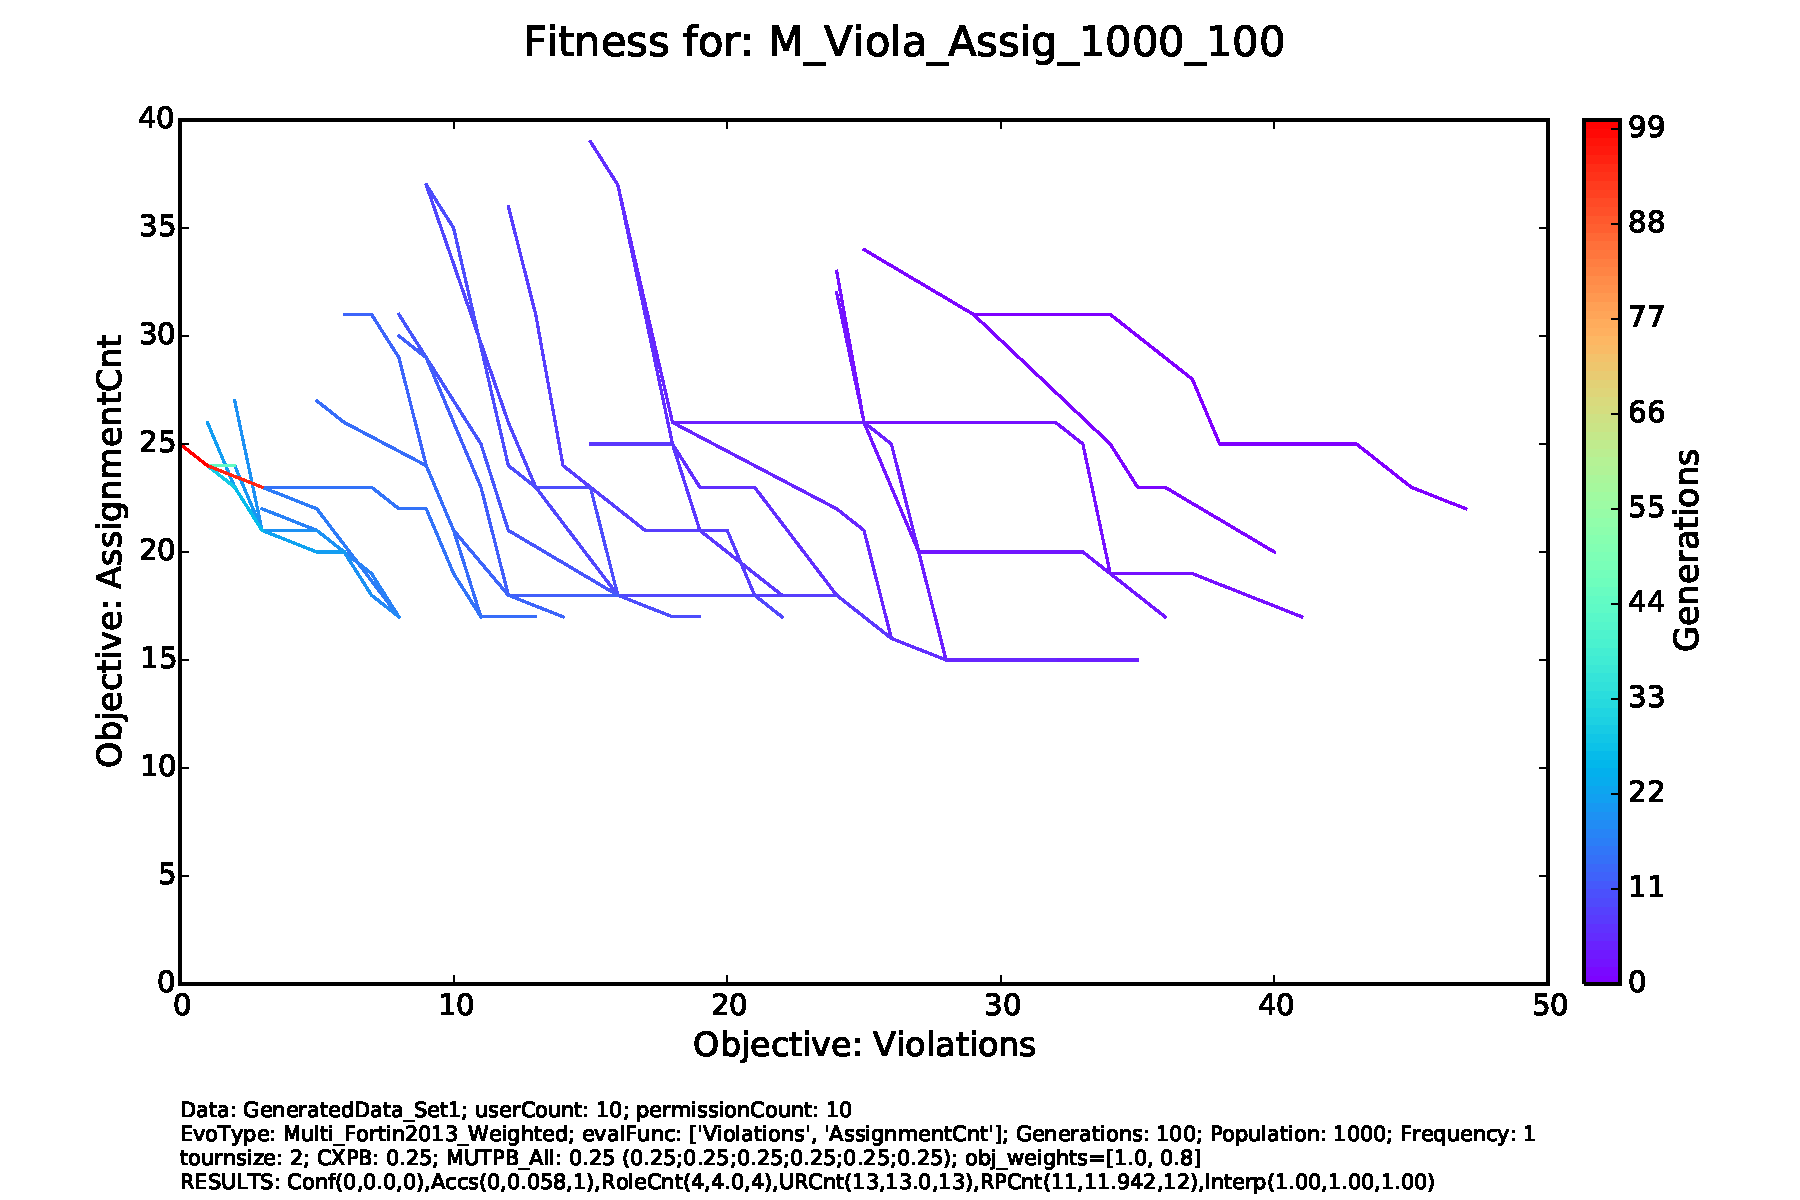
\includegraphics[width=0.8\textwidth, trim=0cm 2cm 0cm 1.5cm, clip=true]{exp4c_fitness_pareto}
		\caption{}
		\label{fig:exp4c_fitness_B}
	\end{subfigure}
	\caption{EXPERIMENT 4c: Example of result of the experiments with Evo-RoleMiner$M$ version 3 on Dataset1. (a) Fitness of individuals over several generations (b) Pareto fronts of each generation.}
	\label{fig:exp4c_fitness}
\end{figure}

The development of the pareto front over the generations (see Figure \ref{fig:exp4c_fitness}) with the third version of the Evo-RoleMiner$M$ looks different than development of the pareto fronts in the other versions of the Evo-RoleMiner$M$ (see Figure \ref{fig:exp4a_fitness} and \ref{fig:exp4b_fitness}). This is due to the stochastic version of pareto dominance (see section \ref{sec:weightedNSGA2}).